\chapter{Experiments with the framework}
The purpose of this chapter is to test our framework.
We start by better defining the concept of \textit{balance} for the purpose of our research and by ensuring that the bot profiles defined and the weapons they use are balanced.
We then proceed to describe a new map representation, \textit{Grid-graph}, that will be used as a possible replacement for \textit{All-black}.

Using this new representation, we will run some evolutionary experiments with the purpose of obtaining maps capable of restoring balance in a situation of skill gap between players.

\label{section:bot_balance}
\section{Bot balance}

In order to use the profiles defined in the previous chapters for the experiments, we first have to verify that they are \textit{balanced}. Defining what balanced means isn't trivial, and requires defining a context. Consider for example a match between an extremely skilled \textit{Sniper} versus a rookie \textit{Shotgun}. What would be a \textit{balanced} result for a match? An equal number of kills and deaths for the bots might \textit{seem} balanced, but what if the map consists only of long, narrow corridors? In such scenarios, greatly favouring a sniper profile, it would be extremely suspicious if a weak shotgun profile were able to obtain a 1/1 kill-death ratio, hinting that the profiles aren't probably balanced.

\begin{figure}[hbtp]

\centering
\begin{subfigure}[t]{0.3\textwidth}
	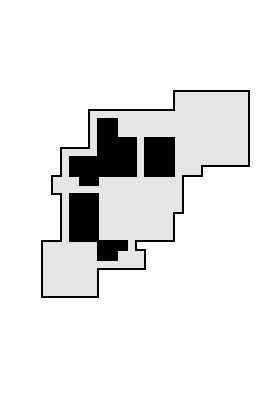
\includegraphics[width=\linewidth]{Images/images/heatmaps/map_generic.png}
	\label{fig:generic_map}
	\caption{The generic map.}
\end{subfigure}
~
\centering
\begin{subfigure}[t]{0.3\textwidth}
	
\includegraphics[width=\linewidth]{Images/images/heatmaps/map_corridor.png}
	\label{fig:corridor_map}
	\caption{The corridor map.}
\end{subfigure}
~
\centering
\begin{subfigure}[t]{0.3\textwidth}
	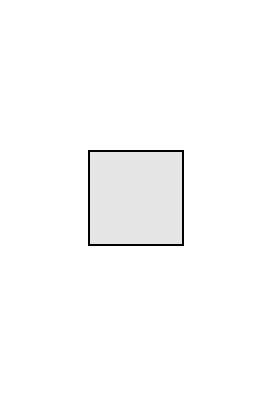
\includegraphics[width=\linewidth]{Images/images/heatmaps/map_arena.png}
	\label{fig:arena_map}
	\caption{The arena map.}
\end{subfigure}
~
\caption{Maps used for our balancing experiments.}
\end{figure}

Given this considerations and the fact that, unlike Arnaboldi and Cube 2 \citep{arnaboldi_framework}, we do not have any pre-made and pre-tested map to use, we opted to test our profiles on three different maps:
\begin{itemize}
\item \textbf{Generic}: A generic map offering oppurtunities for both close, mid and long ranged combats (\Cref{fig:generic_map}).
\item \textbf{Corridor}: A map favouring long-range combat taken to the extreme, consisting of an extremely linear map with no space to dodge projectiles (\Cref{fig:arena_map}).
\item \textbf{Arena}: A map favouring close-range combat taken to the extreme, consisting of a single arena (\Cref{fig:arena_map}).
\end{itemize}

Figures \ref{fig:begin_balance_heatmaps} to \ref{fig:end_balance_heatmaps} show the result of our balance analysis through the use of heatmaps, representing the kill ratio (expressed as \textit{log2}) and absolute kill difference between the two profiles. 
For every matchup, we run different simulations changing the general skill parameter of the two profiles in steps of 0.025.

\subsection{Same profile balance}
Here we show the fight balance for fights between bots with the same profile, but different skill score, on the \textit{generic} map. This can help us validate that changing the skill score has a tangible effect on the capabilities of the bot.

\begin{figure}[H]
    \centering
    \begin{subfigure}[t]{0.5\textwidth}
        \centering
        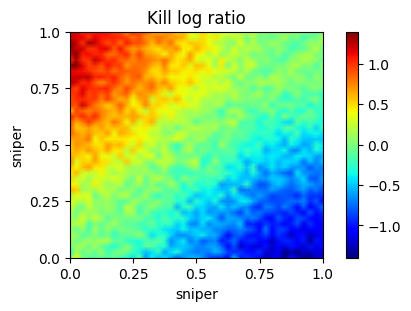
\includegraphics[height=5cm]{Images/images/heatmaps/same-profile/sniper_heatmap_ratio.png}
    \end{subfigure}%
    ~ 
    \begin{subfigure}[t]{0.5\textwidth}
        \centering
        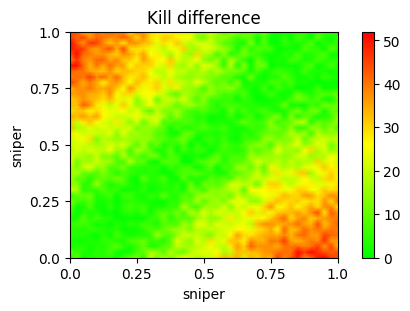
\includegraphics[height=5cm]{Images/images/heatmaps/same-profile/sniper_heatmap_diff.png}
    \end{subfigure}
    \caption{Heatmaps for the \textit{Sniper} vs \textit{Sniper} matchup.}
    \label{fig:balance_sniper_sniper}
    \label{fig:begin_balance_heatmaps}
\end{figure}

\begin{figure}[H]
    \centering
    \begin{subfigure}[t]{0.5\textwidth}
        \centering
        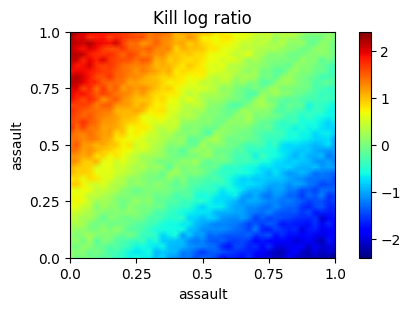
\includegraphics[height=5cm]{Images/images/heatmaps/same-profile/assault_heatmap_ratio.png}
    \end{subfigure}%
    ~ 
    \begin{subfigure}[t]{0.5\textwidth}
        \centering
        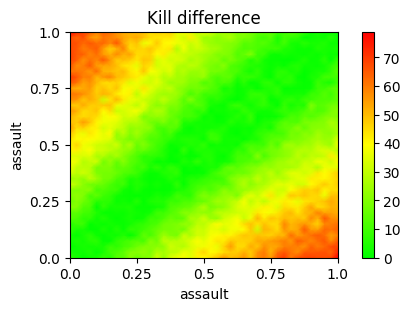
\includegraphics[height=5cm]{Images/images/heatmaps/same-profile/assault_heatmap_diff.png}
    \end{subfigure}
    \caption{Heatmaps for the \textit{Assault} vs \textit{Assault} matchup.}
    \label{fig:balance_assault_assault}
\end{figure}

\begin{figure}[H]
    \centering
    \begin{subfigure}[t]{0.5\textwidth}
        \centering
        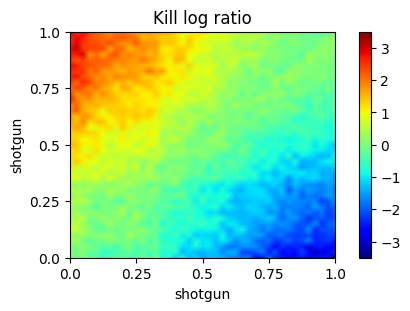
\includegraphics[height=5cm]{Images/images/heatmaps/same-profile/shotgun_heatmap_ratio.png}
    \end{subfigure}%
    ~ 
    \begin{subfigure}[t]{0.5\textwidth}
        \centering
        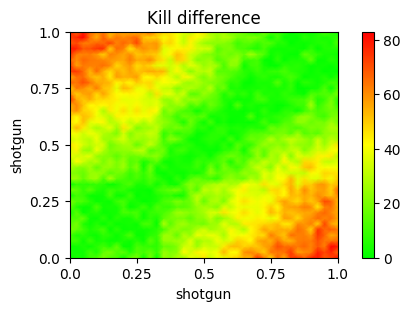
\includegraphics[height=5cm]{Images/images/heatmaps/same-profile/shotgun_heatmap_diff.png}
    \end{subfigure}
    \caption{Heatmaps for the \textit{Shotgun} vs \textit{Shotgun} matchup.}
    \label{fig:balance_shotgun_shotgun}
\end{figure}

From this first balancing experiment we can verify that changing the \textit{general skill} has a noticeable effect on the capabilities of the bot and bots with higher general skill are able to achieve better results against lower skilled opponents.
We can also notice how the \textit{Shotgun} profile is the most influenced by the skill parameter, since it is the one capable of achieving the highest kill ratio and absolute kill difference. This is likely related to the fact that the \textit{Shotgun} is the weapon with the highest \textit{Damage Per Second} in the game and it is therefore capable, in the right hand, to score more kills in the time allotted. Conversely, the \textit{Sniper} is the one showing the smallest difference between skilled and unskilled player, probably for similar reasons.

\subsection{Arena map balance}

In the \textit{Arena} map, as expected, the \textit{Shotgun} profile is the one capable of achieving the best results against the other two profiles, managing to hold its ground even when fighting stronger opponents in terms of skill.

We can also notice how the \textit{Sniper} profile isn't able to shine particularly, not even at the highest levels of skill, as expected due to the limited size of the map.

\begin{figure}[H]
    \centering
    \begin{subfigure}[t]{0.5\textwidth}
        \centering
        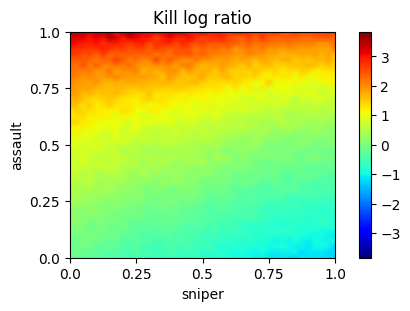
\includegraphics[height=5cm]{Images/images/heatmaps/short-range/assault_sniper_heatmap_ratio.png}
    \end{subfigure}%
    ~ 
    \begin{subfigure}[t]{0.5\textwidth}
        \centering
        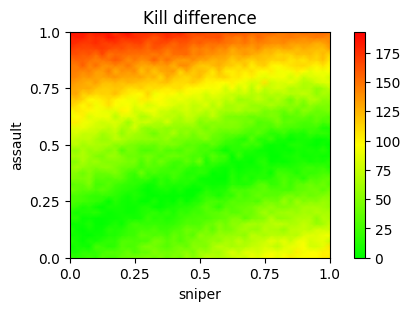
\includegraphics[height=5cm]{Images/images/heatmaps/short-range/assault_sniper_heatmap_diff.png}
    \end{subfigure}
    \caption{Heatmaps for the \textit{Assault} vs \textit{Sniper} matchup.}
    \label{fig:balance_assault_sniper_short}
\end{figure}

\begin{figure}[H]
    \centering
    \begin{subfigure}[t]{0.5\textwidth}
        \centering
        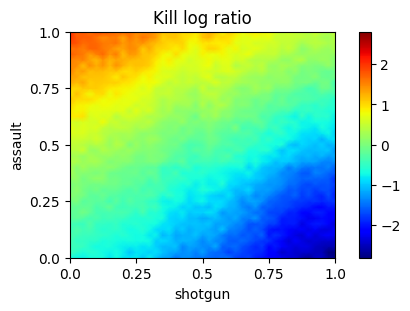
\includegraphics[height=5cm]{Images/images/heatmaps/short-range/assault_shotgun_heatmap_ratio.png}
    \end{subfigure}%
    ~ 
    \begin{subfigure}[t]{0.5\textwidth}
        \centering
        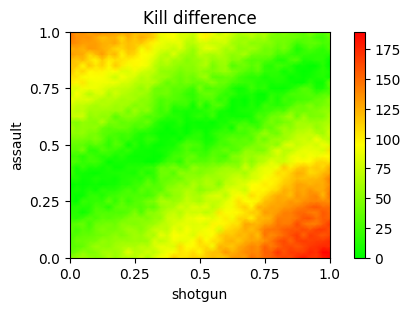
\includegraphics[height=5cm]{Images/images/heatmaps/short-range/assault_shotgun_heatmap_diff.png}
    \end{subfigure}
    \caption{Heatmaps for the \textit{Assault} vs \textit{Shotgun} matchup.}
    \label{fig:balance_assault_shotgun_short}
\end{figure}

\begin{figure}[H]
    \centering
    \begin{subfigure}[t]{0.5\textwidth}
        \centering
        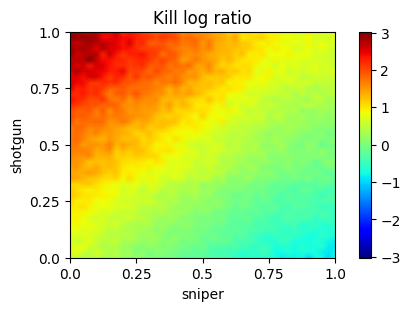
\includegraphics[height=5cm]{Images/images/heatmaps/short-range/shotgun_sniper_heatmap_ratio.png}
    \end{subfigure}%
    ~ 
    \begin{subfigure}[t]{0.5\textwidth}
        \centering
        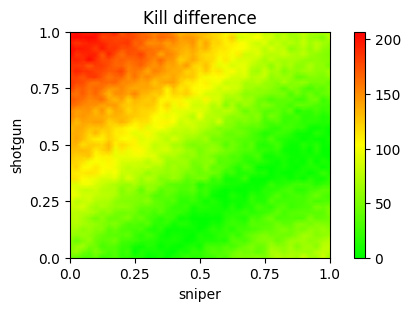
\includegraphics[height=5cm]{Images/images/heatmaps/short-range/shotgun_sniper_heatmap_diff.png}
    \end{subfigure}
    \caption{Heatmaps for the \textit{Shotgun} vs \textit{Sniper} matchup.}
    \label{fig:balance_shotgun_sniper_short}
\end{figure}

\subsection{Generic map balance}
For the \textit{Generic} map, we can see that the situation is more or less balanced for all matchups, except the \textit{Sniper} vs \textit{Shotgun} matchup which shows a little disadvantage for the \textit{Sniper}. This doesn't necessarily mean that the \textit{Sniper} profile is weaker in general, the map might be favouring slightly the \textit{Shotgun}.

\begin{figure}[H]
    \centering
    \begin{subfigure}[t]{0.5\textwidth}
        \centering
        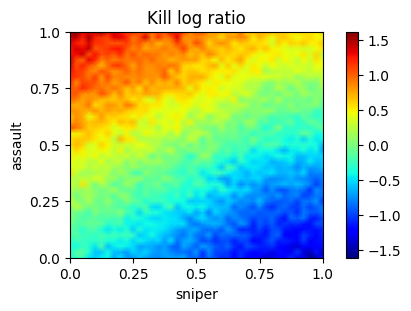
\includegraphics[height=5cm]{Images/images/heatmaps/mid-range/assault_sniper_heatmap_ratio.png}
    \end{subfigure}%
    ~ 
    \begin{subfigure}[t]{0.5\textwidth}
        \centering
        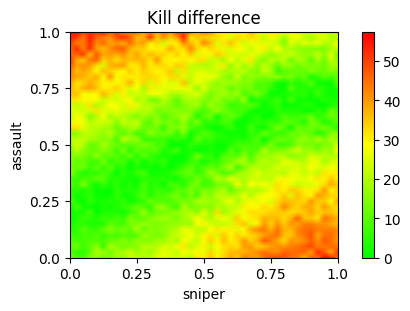
\includegraphics[height=5cm]{Images/images/heatmaps/mid-range/assault_sniper_heatmap_diff.png}
    \end{subfigure}
    \caption{Heatmaps for the \textit{Assault} vs \textit{Sniper} matchup.}
    \label{fig:balance_assault_sniper_mid}
\end{figure}

\begin{figure}[H]
    \centering
    \begin{subfigure}[t]{0.5\textwidth}
        \centering
        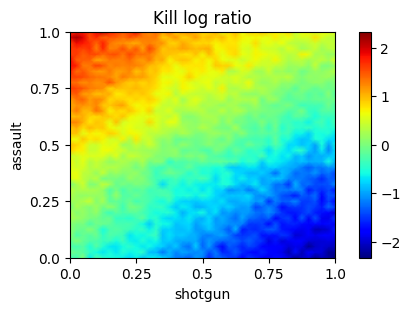
\includegraphics[height=5cm]{Images/images/heatmaps/mid-range/assault_shotgun_heatmap_ratio.png}
    \end{subfigure}%
    ~ 
    \begin{subfigure}[t]{0.5\textwidth}
        \centering
        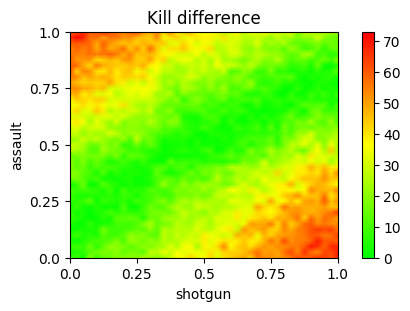
\includegraphics[height=5cm]{Images/images/heatmaps/mid-range/assault_shotgun_heatmap_diff.png}
    \end{subfigure}
    \caption{Heatmaps for the \textit{Assault} vs \textit{Shotgun} matchup.}
    \label{fig:balance_assault_shotgun_mid}
\end{figure}

\begin{figure}[H]
    \centering
    \begin{subfigure}[t]{0.5\textwidth}
        \centering
        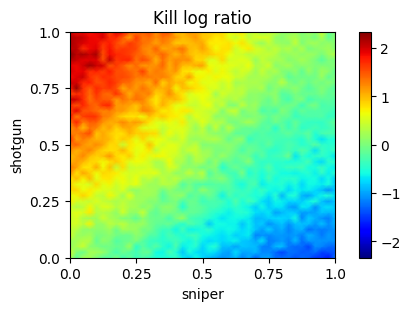
\includegraphics[height=5cm]{Images/images/heatmaps/mid-range/shotgun_sniper_heatmap_ratio.png}
    \end{subfigure}%
    ~ 
    \begin{subfigure}[t]{0.5\textwidth}
        \centering
        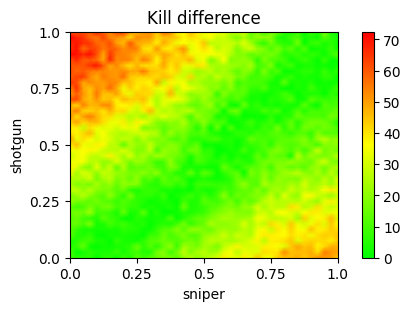
\includegraphics[height=5cm]{Images/images/heatmaps/mid-range/shotgun_sniper_heatmap_diff.png}
    \end{subfigure}
    \caption{Heatmaps for the \textit{Shotgun} vs \textit{Sniper} matchup.}
    \label{fig:balance_shotgun_sniper_mid}
\end{figure}

%###############

\subsection{Corridor map balance}

Finally, in the \textit{Corridor} map, we can see, as expected, that the \textit{Sniper} profile is able, even at the lowest skill level, to defeat the other two profiles and, in the matchup against the \textit{Shotgun}, by a wide margin,
Interestingly enough however, the \textit{Assault} rifle is the one capable of achieving the best kill ratio (8/1) against the \textit{Shotgun} profile. This is likely caused by the higher DPS of the \textit{Assault} rifle, which allows the wielder to dispatch opponents faster.

\begin{figure}[H]
    \centering
    \begin{subfigure}[t]{0.5\textwidth}
        \centering
        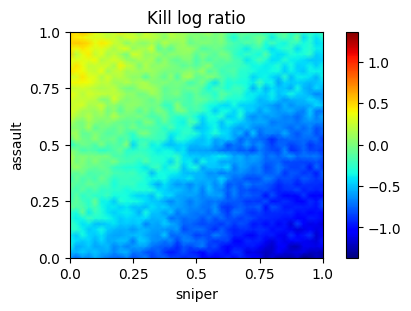
\includegraphics[height=5cm]{Images/images/heatmaps/long-range/assault_sniper_heatmap_ratio.png}
    \end{subfigure}%
    ~ 
    \begin{subfigure}[t]{0.5\textwidth}
        \centering
        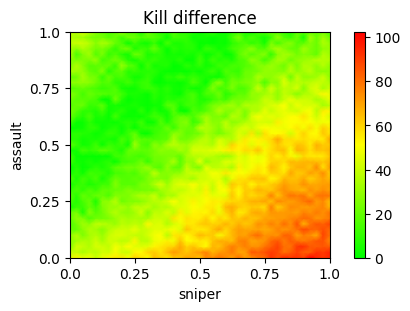
\includegraphics[height=5cm]{Images/images/heatmaps/long-range/assault_sniper_heatmap_diff.png}
    \end{subfigure}
    \caption{Heatmaps for the \textit{Assault} vs \textit{Sniper} matchup.}
    \label{fig:balance_assault_sniper_long}
\end{figure}

\begin{figure}[H]
    \centering
    \begin{subfigure}[t]{0.5\textwidth}
        \centering
        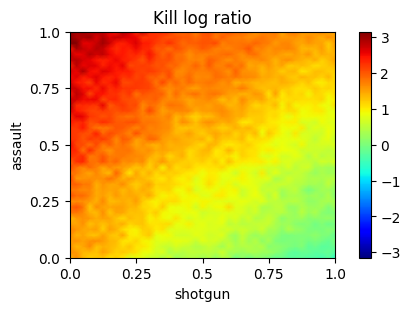
\includegraphics[height=5cm]{Images/images/heatmaps/long-range/assault_shotgun_heatmap_ratio.png}
    \end{subfigure}%
    ~ 
    \begin{subfigure}[t]{0.5\textwidth}
        \centering
        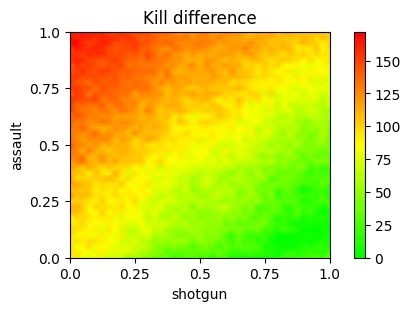
\includegraphics[height=5cm]{Images/images/heatmaps/long-range/assault_shotgun_heatmap_diff.png}
    \end{subfigure}
    \caption{Heatmaps for the \textit{Assault} vs \textit{Shotgun} matchup.}
    \label{fig:balance_assault_shotgun_long}
\end{figure}

\begin{figure}[H]
    \centering
    \begin{subfigure}[t]{0.5\textwidth}
        \centering
        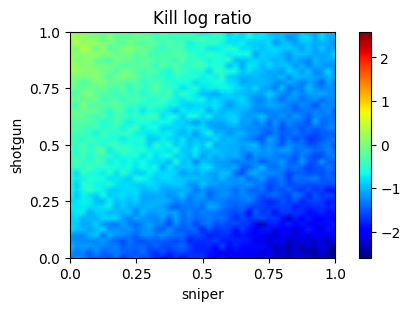
\includegraphics[height=5cm]{Images/images/heatmaps/long-range/shotgun_sniper_heatmap_ratio.png}
    \end{subfigure}%
    ~ 
    \begin{subfigure}[t]{0.5\textwidth}
        \centering
        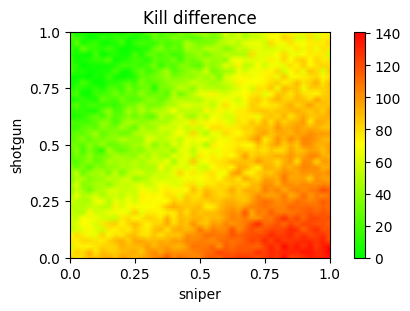
\includegraphics[height=5cm]{Images/images/heatmaps/long-range/shotgun_sniper_heatmap_diff.png}
    \end{subfigure}
    \caption{Heatmaps for the \textit{Shotgun} vs \textit{Sniper} matchup.}
    \label{fig:balance_shotgun_sniper_long}
    \label{fig:end_balance_heatmaps}
\end{figure}

\section{Grid-graph map representation}
In this section we describe the original \textit{All-black} representation used in the framework, analyse some of its shortcomings and propose a new representation \textit{Grid-graph}, on top of which the different evolutionary experiments will be run.

\subsubsection{Limits of the original models}
Many of the researches performed on evolution of maps for first person shooter used as their basis the map genotypes developed by Cardamone \citep{cardamone_evolving_maps}. Among the four proposed representations, \textit{Grid}, \textit{All-white}, \textit{All-black} and \textit{Random-Digger}, \textit{All-white} was the one capable of producing the maps with the highest fitness, but the produced result look bland and lack any notable feature.
The \textit{All-black} representation on the other hand, despite performing worse on average, managed to create maps which strongly resemble those produced by level designer, thanks to their emphasis on arenas and corridors, and was therefore chosen as the basis for other researches, such as Arnaboldi's \citep{arnaboldi_framework}. 

We have analysed the \textit{All-black} representation to try to understand why it under performed in the settings of an evolutionary algorithms with exploration of the search space and found two major problems.

The first of this problems is the \textbf{redundancy}. \Cref{fig:all_black_connected} shows an example of the problem: in this genotype, one of the rooms, specifically \textit{<4,3,2>}, is redundant, since it's completely contained in room \textit{<4,4,4>}. Only considering these two rooms, the smallest one can be placed in 8 other positions and still have no effect on the final phenotype. This redundancy problem leads to an exponential increase in the size of the search space, which in turn slows down convergence of any search algorithm employed.

The second problem is the \textbf{lack of locality}, two very similar genotypes can produce substantially different phenotypes, making it difficult for the exploration algorithm to understand how to optimize the fitness function. An example of this phenomenon is presented in \Cref{fig:all_black_disconnected}: a map obtained by simply changing two numbers of the genotype represented in \Cref{fig:all_black_connected}. While one of the changes leads to a negligible variation in the phenotype, the other completely alters the connectivity of the map, greatly affecting the way the map is played.

\begin{figure}
\centering
\captionsetup[subfigure]{}
\subfloat[\centering All-black initial representation]{
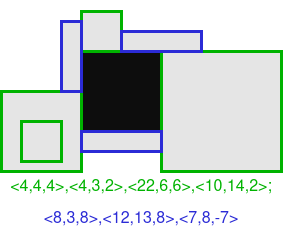
\includegraphics[scale=0.7]{Images/images/ABConnected.png}
\label{fig:all_black_connected}
} 
\subfloat[\centering All-black representation after two small changes]{
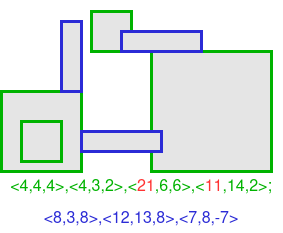
\includegraphics[scale=0.7]{Images/images/ABDisconnected.png}
\label{fig:all_black_disconnected}
} 

\caption{Examples of two All-black representations}
\end{figure}

\subsection{Graph-based map representation: Grid-graph}
In this thesis we propose a graph-based genotype representation for maps, named \textit{Grid-graph}, which should overcome the limitations of the \textit{All-black} representation while still maintaining a lot of similarities and ease of use. 

The \textit{Grid-graph} map representation follows the same approach used by \textit{All-black} and starts with an initial map full of wall blocks and gradually adds space in search of fitter maps.

To place free space, \textit{Grid-graph} starts by subdividing the area into an $R \times C$ grid of equally sized cells, each one occupying $r \times c$ squares. A cell contains zero or one \textbf{Room}, representing a rectangular, axis-aligned, walkable portion of the map. Each room is defined by four values:
\begin{itemize}
\item[w] The width of the \textit{Room}, between 1 and $c$.
\item[h] The height of the \textit{Room}, between 1 and $r$.
\item[x] The x coordinate of the bottom left corner of the \textit{Room} inside the cell, between 0 and $c-w-1$. 
\item[y] The y coordinate of the bottom left corner of the \textit{Room} inside the cell, between 0 and $r-h-1$.
\end{itemize}
To represent the contents of each cell, the genome contains an $R \times C$ matrix where element $(i,j)$ contains the quartet described above if the cell in position $(i,j)$ contains a \textit{Room} or a special value \textit{Nil} in case no \textit{Room} is placed in that cell\footnote{It is possible for this genome to represent maps which do not contain any free space. When that happens, the genome should simply be discarded.}.

\textit{Rooms} placed in vertically or horizontally adjacent cells can be connected by a \textbf{Corridor}. Each corridor is simply represented as a boolean value \textit{<b>} indicating whether the two adjacent rooms (if present) must be connected. All the horizontal corridors are saved in a $R \times (C-1)$ matrix, where the boolean at position $(i,j)$ represents whether \textit{Rooms} $(i,j)$, $(i,j+1)$ are connected and similarly all the vertical corridors are stored in an $(R-1) \times C$ matrix, where the boolean at position $(i,j)$ represents whether \textit{Rooms} $(i,j)$, $(i+1,j)$ are connected.

\textit{Corridors} do not have any specified size or shape defined in the genotype, rather, they are generated dynamically to connect the various rooms depending on the placement of them. For example, two rooms which are not aligned must be connected by a corridor with a bend in the middle, or again, two rooms adjacent by at least one square do not need a corridor at all and are simply fused together. 

When converting the genome to it's actual map representation, it possible to run into a problem: the resulting map might be disconnected. This problem was already identified by Cardamone \cite{cardamone_evolving_maps} for other map representations and we will be using the same approach adopted in his research: in case of multiple disjointed connected components, the one closest to the center is selected and the other parts of the map are ignored.

An example of \textit{Grid-graph} genome and related phenotype are shown in \Cref{fig:grid-graph-genome-phenotype}.

\begin{figure}[hbtp]
\centering
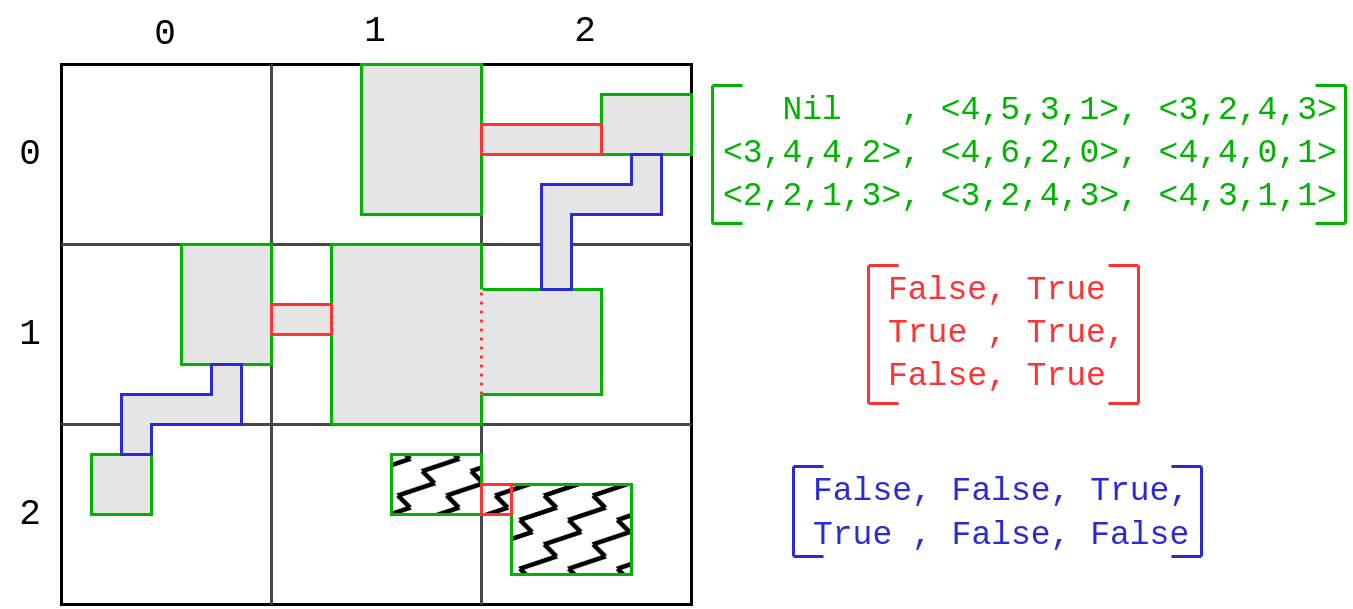
\includegraphics[width=0.9\linewidth]{Images/images/Grid-graph.png}
\caption{Example of Grid-graph phenotype and related genotype. \textcolor{green}{Rooms} are shown in green, \textcolor{red}{horizontal corridors} in red and \textcolor{blue}{vertical corridors} in blue. The parts of the map disconnected are filled with a zig-zagged line}
\label{fig:grid-graph-genome-phenotype}
\end{figure}

\begin{figure}
\centering
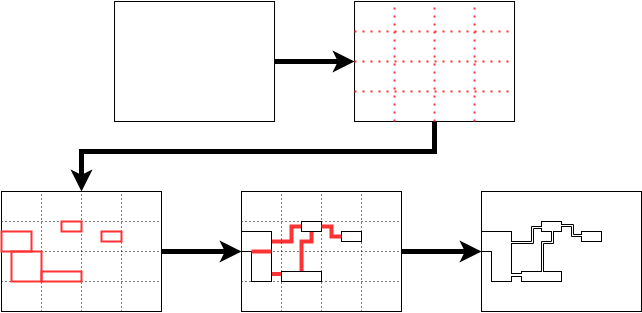
\includegraphics[scale=0.6]{Images/images/MapGeneration.drawio.png}  
\caption{Generation process for a Grid-graph map}
\label{fig:grid-graph-generation}
\end{figure}

\subsubsection{Comparison between All-black and Grid-graph}
The \textit{Grid-graph} map representation tries to maintain some of the key concepts used in the \textit{All-black} representation and refines others. 

\textit{Rooms} for example are virtually identical between the two representations and the most notable difference is that in \textit{Grid-graph} their placement is not completely free, since each room must be placed in a cell and only one \textit{Room} can be contained in each cell.

\textit{Corridors} instead have been completely revamped: while in \textit{All-black} a corridor is just a non-square room, in \textit{Grid-graph} corridors have a proper function: connecting different rooms. This greatly simplifies maps, since connecting non-aligned rooms doesn’t require strategically placed corridors as was the case for \textit{All-black}, and make maps more resilient to changes since now two rooms cannot get disconnected by chance, simply because they got resized or moved.

Since \textit{Rooms} and \textit{Corridors} in \textit{Grid-graph} map can be placed only in specific places and overlaps are forbidden, this representation does not incur in same kind of \textit{redundancy} problem prominent in \textit{All-black} maps. 
However, it should be noted that, given the grid layout of \textit{Grid-graph}, maps will tend to look more simple than those obtained with \textit{All-Black}. As an example, consider the map in \Cref{fig:complex_AB_map}. It would be basically impossible for \textit{Grid-graph} to replicate many of the features, such as little nooks and crannies, dead-end corridors, extra walls and so on.
Nonetheless, it's not clear yet the influence that all those little features have on matches, they could be an integral part in what makes a given map great or they could simply be considered "noise" that can be simply discarded.

Regarding the second problem present in \textit{All-black} maps instead, the \textit{lack of locality}, \textit{Grid-graph} maps are also affected by it, but in a more controllable way, since two adjacent regions of the map can be disconnected only if the room or corridor connecting them is removed. With \textit{All-black} instead any modification to any parameter can potentially alter the map topology, be it moving, removing or resizing a room or corridor.

\begin{figure}
\centering
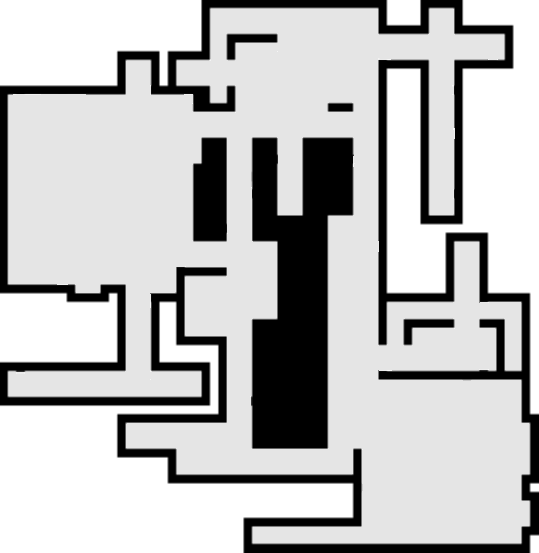
\includegraphics[scale=0.4]{Images/images/random-arnaboldi-map.png}  
\caption{Example of map obtained using All-black representation}
\label{fig:complex_AB_map}
\end{figure}

\section{Evolving new maps: Balance and pacing}
For this experiment we wanted to evolve maps which, starting from a initial situation of unbalance due to the different level of skill of the players involved, tries to evolve maps that result in balanced matches, additionally trying to maximize the \textit{pace}.
We will be running the experiment in two different configurations, one using the \textit{Grid-graph} representation and the other using the \textit{All-black} representation, in order to compare the two. For each experiment we will be executing 8 different runs.

\subsection{Common setup}

The two experiments we will conduct have several parameters in common, starting with the profiles used: \textit{Sniper} and \textit{Shotgun}, summarised in \Cref{table:parameters_first_experiment}, and their respective skill levels of 0.15 and 0.85. For this combination of profiles and skills, the resulting entropy achieved in the experiments conducted on the generic map in in \Cref{section:bot_balance} was approximately 0.84, corresponding to a kill ratio of 2.77 in favour of the \textit{Shotgun}.

\begin{table}
\begin{center}
\begin{tabular}{|| c || c | c ||}
 \hline
 Skill & Shotgun & Sniper \\ 
 \hline 
 Eye speed & 1.2 & 0.8 \\  
 Reflex & 0.9 & 1.3 \\   
 Prediction & 1.1 & 0.7 \\  
 Aim & 0.6 & 1.15 \\  
 Movement & 1.2 & 0.6 \\  
 Curiosity & High & Low \\  
 Recklessness & High & Low \\  
 Max Range & 50 & 200 \\  
 Speed & 20 & 20 \\  
 \hline
\end{tabular}
\caption{Different bot profiles defined for our experiments}
\label{table:parameters_first_experiment}
\end{center}
\end{table}

Both experiments will involve populations consisting of 52 individuals, spanning across 30 generations, and will utilize a multi-objective fitness approach in conjunction with the NSGA-II selection algorithm \cite{ngsaII}. 

Any time the algorithm needs to run a match between the bots, two game simulations, lasting 20 minutes each, are launched and the final results, used to compute the fitness, are averaged. This was done in order to reduce any potential error caused by the stochastic nature of the bots and of the simulations.

\subsection{Grid-graph experiment}
For our first experiment, we will test how suitable the \textit{Grid-graph} representation is in the context of evolutionary algorithms.

We will use a map composed of an 8x8 grid of cells, evolved using as \textit{crossover} operation a simple matrix crossover (given the grid nature of the map) with probability $0.3$ and as \textit{mutation} operator a two-points mutation with probability 0.3.

\Cref{fig:ex_one_pareto_area} shows the evolution of the area under the Pareto front for the first 30 generations of the evolutionary process, averaged across the runs.
Looking at the picture, we can observe a continuous expansion of the Pareto front area during the whole process, but the increase per epoch slows down drastically after the fifteenth generation. Considering the whole process, the average area under the Pareto front grew by 12\%.

\begin{figure}[hbtp]
\centering
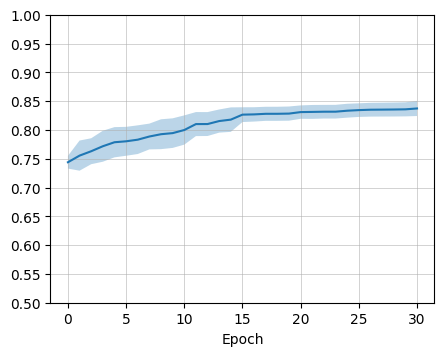
\includegraphics[width=0.5\linewidth]{Images/images/experiment_one/Pareto/pareto_evolution_avg.png}
\caption{Evolution of the area under the Pareto front}
\label{fig:ex_one_pareto_area}
\end{figure}

\begin{figure}[hbtp]
    \centering
    \begin{subfigure}[t]{0.5\textwidth}
        \centering
        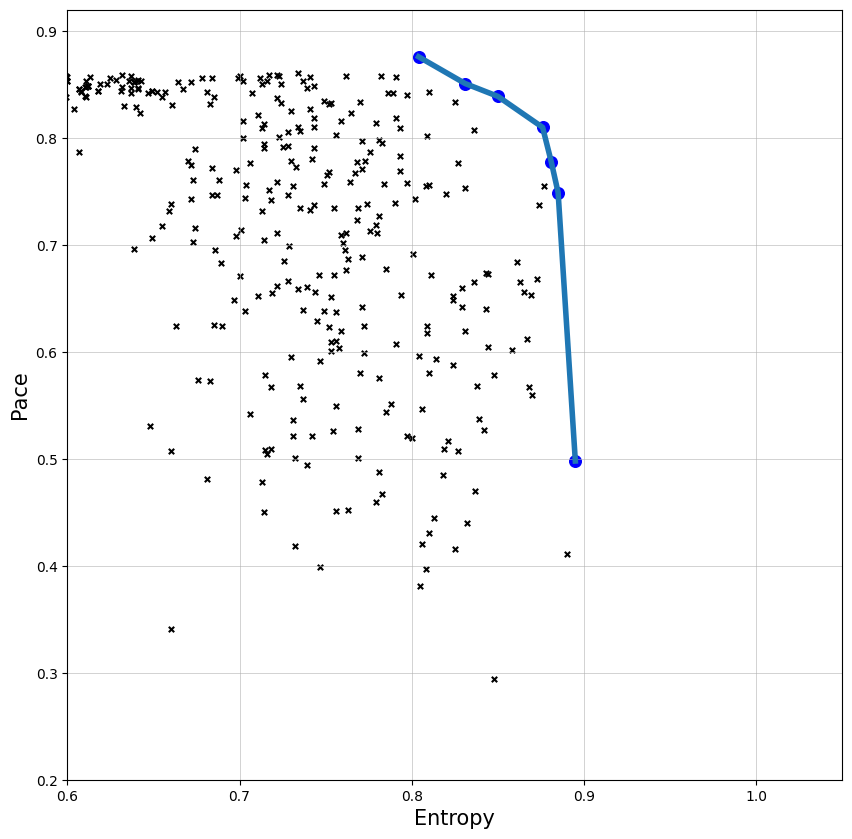
\includegraphics[height=7cm]{Images/images/experiment_one/Pareto/pareto_front_total_begin.png}
        \caption{Initial Pareto front.}
    \end{subfigure}%
    ~ 
    \begin{subfigure}[t]{0.5\textwidth}
        \centering
        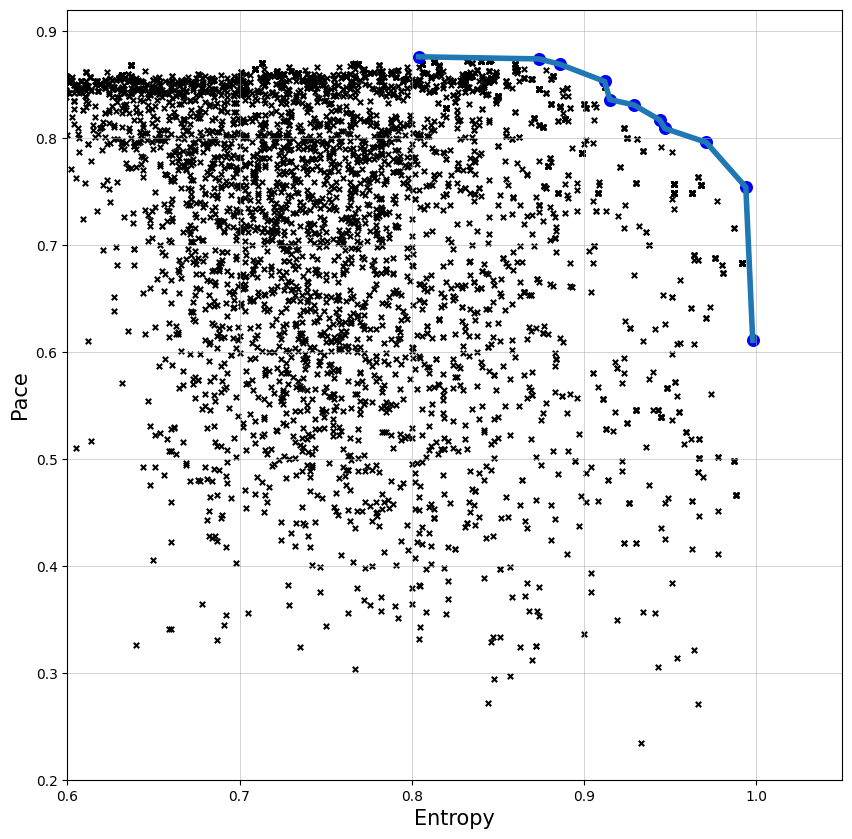
\includegraphics[height=7cm]{Images/images/experiment_one/Pareto/pareto_front_total_final.png}
        \caption{Final Pareto front.}
        \label{fig:ex_one_final_pareto_total}
    \end{subfigure}
    \caption{Evolution of the Pareto front.}
    \label{fig:ex_one_pareto_evolution}
\end{figure}


\begin{figure}[hbtp]
    \centering
    \begin{subfigure}[t]{0.5\textwidth}
        \centering
        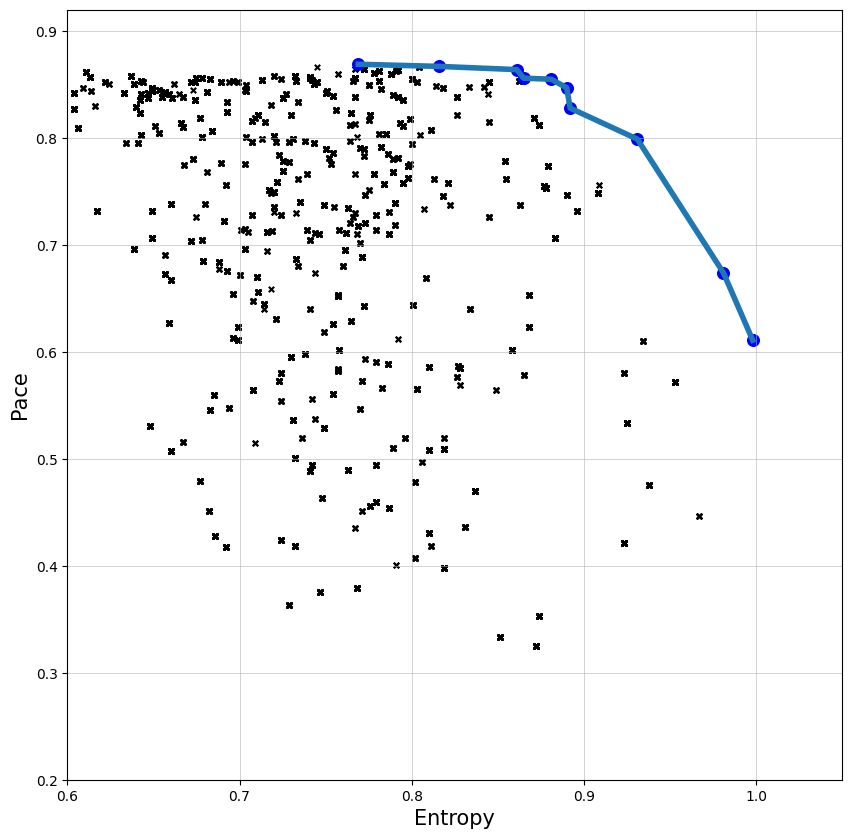
\includegraphics[height=7cm]{Images/images/experiment_one/Pareto/pareto_front_population_0.png}
    \end{subfigure}%
    ~ 
    \begin{subfigure}[t]{0.5\textwidth}
        \centering
        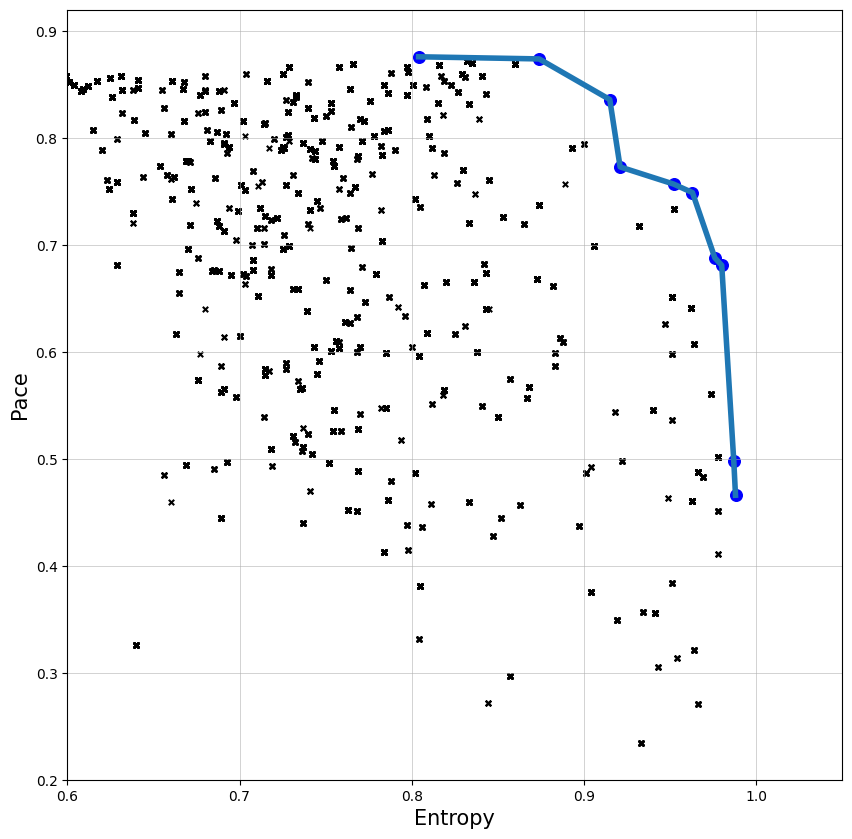
\includegraphics[height=7cm]{Images/images/experiment_one/Pareto/pareto_front_population_1.png}
    \end{subfigure}
    \caption{Pareto front of 2 of the 8 runs.}
    \label{fig:ex_one_pareto_populations}
\end{figure}


\Cref{fig:ex_one_pareto_evolution} allows us to compare the Pareto front at the start and end of the evolutionary process. It's evident that there hasn't been a significant increase in \textit{pace}, but in terms of \textit{entropy}, there has been a noticeable shift from a maximum value of approximately 0.9 to a value close to 1 (0.998), or, in terms of kill ratio, a decrease from 2.1 to 1.1.

The unsatisfactory improvements in \textit{pace} can be attributed to a simple consideration: a \textit{pace} value of $0.9$ corresponds to a combat every second, a rate that cannot be further improved due to the time it takes for bots to respawn and react to enemies. 
\Cref{fig:best_pace_map_0} and \Cref{fig:best_pace_map_1} show the best maps, in terms of \textit{pace}, for two of the eight simulations run. These two maps look extremely bland, they just consist of a single room, offering no cover or escape, therefore forcing combat immediately every time.

In contrast, the improvements in \textit{entropy} are much more promising, especially when considering its logarithmic trend. A value of 0.9 corresponds to a kill-death ratio of around $2.2$ in favor of the \textit{Shotgun} profile, while a unitary value indicates a perfect balance between the bots. An almost perfect balance was achieved by the map shown in \Cref{fig:best_entropy_map_0}.

The distribution of values in \Cref{fig:ex_one_final_pareto_total} shows a concentration of individuals having high pace values and average entropy values, but there are also plenty of other individuals scattered around, hinting that a big portion of the search space was explored during the evolution.

Lastly, it's noticeable that while for average \textit{entropy} values the evolutionary algorithm has always been able to find maps that maximize \textit{pace}, with entropy values tending towards 1, there is a sudden reversal of this trend, leading, at the extreme, to a pace value as low as $0.46$. This behavior can be reasonably explained by considering that those maps which maximize \textit{entropy} tend to be highly elongated, increasing the time it takes for bots to find each other and start combat.

%\begin{figure}[hbtp]
%    \centering
%    \begin{subfigure}[t]{0.3\textwidth}
%        \centering
%        
\includegraphics[height=4.5cm]{Images/images/experiment_one/best_entropy_total/map.png}
%        \caption{Map with entropy 0.999 and pace 0.689.}
%        \label{fig:ex_one_map_entropy}
%    \end{subfigure}%
%    ~ 
%    \begin{subfigure}[t]{0.3\textwidth}
%        \centering
%        
\includegraphics[height=4.5cm]{Images/images/experiment_one/best_fitness_total/map.png}
%        \caption{Map with entropy 0.992 and pace 0.775.}
%    \end{subfigure}
%    ~ 
%    \begin{subfigure}[t]{0.3\textwidth}
%        \centering
%        
\includegraphics[height=4.5cm]{Images/images/experiment_one/best_pace_total/map.png}
%        \caption{Map with entropy 0.729 and pace 0.897}
%        \label{fig:ex_one_map_pace}
%    \end{subfigure}
%    \caption{Maps maximising entropy, pace and fitness considering all populations combined.}
%    \label{fig:ex_one_pareto_evolution_combined}
%\end{figure}

\begin{figure}[hbtp]
    \centering
    \begin{subfigure}[t]{0.3\textwidth}
        \centering
        
\includegraphics[height=4.5cm]{Images/images/experiment_one/best_entropy_pop_0/map.png}
        \caption{Map with entropy 0.998 and pace 0.611.}
        \label{fig:best_entropy_map_0}
    \end{subfigure}%
    ~ 
    \begin{subfigure}[t]{0.3\textwidth}
        \centering
        
\includegraphics[height=4.5cm]{Images/images/experiment_one/best_fitness_pop_0/map.png}
        \caption{Map with entropy 0.981 and pace 0.674.}    
        \label{fig:best_fitness_map_0}
    \end{subfigure}
    ~ 
    \begin{subfigure}[t]{0.3\textwidth}
        \centering
        
\includegraphics[height=4.5cm]{Images/images/experiment_one/best_pace_pop_0/map.png}
        \caption{Map with entropy 0.769 and pace 0.869}
        \label{fig:best_pace_map_0}
    \end{subfigure}
    \centering
    \begin{subfigure}[t]{0.3\textwidth}
        \centering
        
\includegraphics[height=4.5cm]{Images/images/experiment_one/best_entropy_pop_1/map.png}
        \caption{Map with entropy 0.988 and pace 0.466.}
        \label{fig:best_entropy_map_1}
    \end{subfigure}%
    ~ 
    \begin{subfigure}[t]{0.3\textwidth}
        \centering
        
\includegraphics[height=4.5cm]{Images/images/experiment_one/best_fitness_pop_1/map.png}
        \caption{Map with entropy 0.963 and pace 0.749.}
        \label{fig:best_fitness_map_1}
    \end{subfigure}
    ~ 
    \begin{subfigure}[t]{0.3\textwidth}
        \centering
        
\includegraphics[height=4.5cm]{Images/images/experiment_one/best_pace_pop_1/map.png}
        \caption{Map with entropy 0.804 and pace 0.876}
        \label{fig:best_pace_map_1}
    \end{subfigure}
    \caption{Maps maximising entropy, fitness and pace considering two of the eight runs.}
    \label{fig:ex_one_maps}
\end{figure}


\subsubsection{Map analysis}
One of the first things that stands out from the displayed maps is the simplicity (not to say banality) of the maps obtained by maximizing pace. It simply consists of one room. On these maps, the high visibility and limited total space result in combat occurring at a very fast and potentially exhausting pace. 

Coincidentally, maps maximing \textit{pace} are those with the lowest \textit{entropy}. This is expected, considering the weapons in play. The \textit{Shotgun} profile in particolar shines in close-range combat and this, coupled with the higher general skill, means that the \textit{Sniper} profile cannot compete.

On the other end of the spectrum, maps that maximize \textit{entropy} feature linear structures that favor long-range combat and limit longitudinal movements, preventing the use of techniques such as strafing to approach enemies while avoiding being hit. Additionally, it is often possible to observe the absence of alternative paths to reach any point on the map, further reducing the possibility of approaching enemy snipers. 

%Finally, when observing maps that maximize \textit{fitness}, it is possible to notice an interesting detail for \Cref{fig:ex_one_map_entropy} and \Cref{fig:ex_one_map_fitness}: the latter can be obtained by stripping away the leftmost part of the former, reducing The structure of the obtained maps more closely resemble that of a single long vertical corridor, which still favours long-range combat but also increases the total visibility, leading to more frequent combats.

\subsubsection{Analysis of the dynamics}
We now proceed to analyse the evolved maps using data gathered by our framework. We will be in particular focusing on:
\begin{itemize}
\item \textbf{Kill and Death Heatmaps}: These graphics will display, for each map, at which points kills and deaths tend to occur more or less frequently.
\item \textbf{Kill traces}: These graphics will display the relative position of bots at each individual kill through a segment whose color will be darker the greater the distance between the two.
\end{itemize} 

These graphics are shown in Figures
\ref{fig:ex_one_begin_heatmaps} to \ref{fig:ex_one_end_heatmaps}.

Except for the maps that maximizes \textit{pace}, which, due to their limited size, do not reveal particularly interesting details on match dynamics, the kill traces of the other maps show two distinct play styles for \textit{Shotgun} and \textit{Sniper} profiles that are reflected in their respective death and kill positions.

In regards to the \textit{Sniper} profile, it is noticeable how kills tend to concentrate in close proximity to walls and in the most extreme positions of the maps, locations that allow the \textit{Sniper} to shoot opponents from a safe distance, but which simultaneously do not provide any possibility of retreat in case of need.

Conversely, the \textit{Shotgun} profile frequently positions itself in the most central and open areas of the maps, taking advantage of its high mobility to close in on opponents while evading incoming fire.

%Looking at the death heatmaps, another interesting observation can be made. While it's expected that deaths are concentrated around the central junctions of the map (simply because it's often necessary to cross them to reach any destination), we can see that \textit{Sniper} deaths are always concentrated in the vicinity, while \textit{Shotgun} deaths are more spread out (this is especially noticeable for the second experiment). This is likely due to the different characteristics of the weapons: as soon as the \textit{Shotgun} profile spots an enemy at a crossroad, they only need a single shot to eliminate them. In contrast, a \textit{Sniper }needs two shots, giving the enemy time to move.

\subsubsection{Relation to other characteristics}
As a final analysis, we wanted to investigate if there were any particular relationships between \textit{entropy} and other characteristics, particularly \textit{pace}, \textit{accuracy}, \textit{sight loss rate} and \textit{number of frags}, across all runs. The results, shown in \Cref{fig:ex_one_entropy_relations}, are not particularly surprising given that the evolutionary process aimed to balance a situation of significant disadvantage for the \textit{Sniper} profile.

We can observe a general increase in the \textit{accuracy} and the number of kills or the \textit{Sniper} profile, while there was a clear decrease in the effectiveness of the \textit{Shotgun}, despite the accuracy remaining rather constant during the process. 

This can be attributed to the shape of the maps, which became increasingly narrow and elongated as \textit{entropy} increased, favoring the \textit{Sniper} profile's accuracy (as the \textit{Shotgun} profile has fewer opportunities to evade bullets) without significantly modifying the \textit{Shotgun}'s accuracy, given that the \textit{Shotgun} is already accurate enough at short distances and the \textit{Sniper} isn't proficient in evading techniques such as \textit{strafing}. The decrease in the number of kills for the \textit{Shotgun} profile follows the reduction in the \textit{pace}, which again is likely caused by their gradual elongation of maps which reduces visibility and engage opportunities.

We can also notice a consistent decrease in \textit{Pace}, which can be attributed to the fact that the \textit{Shotgun} profile prefers smaller and more frenetic maps, whereas the \textit{Sniper} profile prefers longer and more stretched-out maps, which slow down the \textit{pace} of encounters.

% TODO evoluzione area delle mappe?

\begin{figure}[H]
\centering
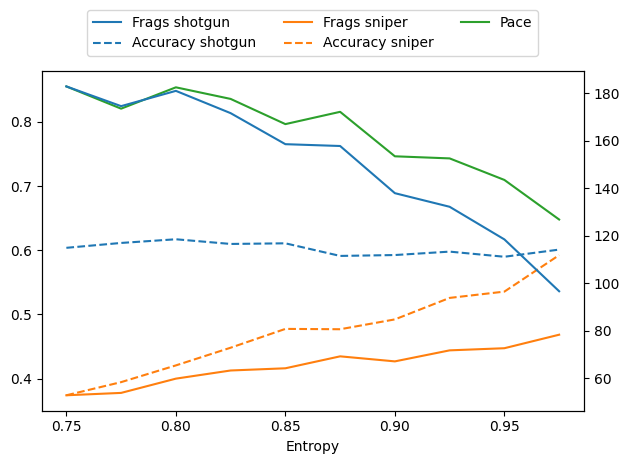
\includegraphics[width=0.6\linewidth]{Images/images/experiment_one/entropy_mix.png}
\caption{Relation of entropy to other characteristics}
\label{fig:ex_one_entropy_relations}
\end{figure}


\newpage

%BEGIN Shotgun first simulation
\begin{figure}[H]
    \centering
    \begin{subfigure}[t]{0.3\textwidth}
        \centering
        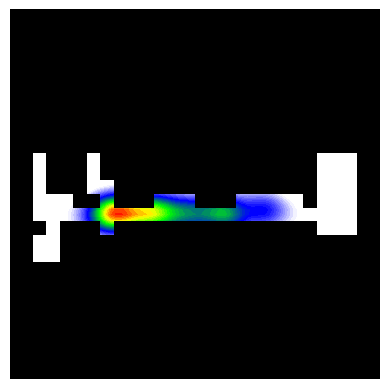
\includegraphics[height=4.5cm]{Images/images/experiment_one/best_entropy_pop_0/deaths_bot_0.png}
        \caption{Map maximising entropy.}
    \end{subfigure}%
    ~ 
    \begin{subfigure}[t]{0.3\textwidth}
        \centering
        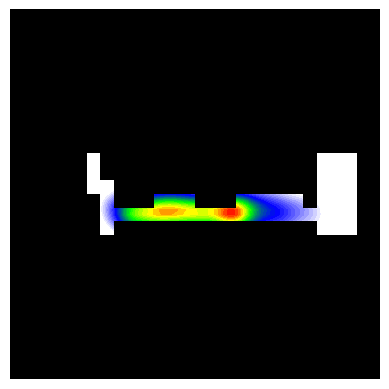
\includegraphics[height=4.5cm]{Images/images/experiment_one/best_fitness_pop_0/deaths_bot_0.png}
        \caption{Map maximising fitness.}
    \end{subfigure}
    ~ 
    \begin{subfigure}[t]{0.3\textwidth}
        \centering
        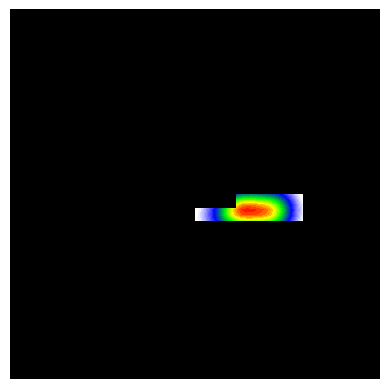
\includegraphics[height=4.5cm]{Images/images/experiment_one/best_pace_pop_0/deaths_bot_0.png}
        \caption{Map maximising pace.}
    \end{subfigure}
    \caption{Heatmaps of the deaths of the Shotgun profile for the first simulation.}
    \label{fig:ex_one_begin_heatmaps}
\end{figure}
\begin{figure}[H]
    \centering
    \begin{subfigure}[t]{0.3\textwidth}
        \centering
        \includegraphics[height=4.5cm]{Images/images/experiment_one/best_entropy_pop_0/kills_bot_0.png}
        \caption{Map maximising entropy.}
    \end{subfigure}%
    ~ 
    \begin{subfigure}[t]{0.3\textwidth}
        \centering
        \includegraphics[height=4.5cm]{Images/images/experiment_one/best_fitness_pop_0/kills_bot_0.png}
        \caption{Map maximising fitness.}
    \end{subfigure}
    ~ 
    \begin{subfigure}[t]{0.3\textwidth}
        \centering
        \includegraphics[height=4.5cm]{Images/images/experiment_one/best_pace_pop_0/kills_bot_0.png}
        \caption{Map maximising pace.}
    \end{subfigure}
    \caption{Heatmaps of the kills of the Shotgun profile for the first simulation.}
\end{figure}
\begin{figure}[H]
    \centering
    \begin{subfigure}[t]{0.3\textwidth}
        \centering
        \includegraphics[height=4.5cm]{Images/images/experiment_one/best_entropy_pop_0/kill_traces_bot_0.png}
        \caption{Map maximising entropy.}
    \end{subfigure}%
    ~ 
    \begin{subfigure}[t]{0.3\textwidth}
        \centering
        \includegraphics[height=4.5cm]{Images/images/experiment_one/best_fitness_pop_0/kill_traces_bot_0.png}
        \caption{Map maximising fitness.}
    \end{subfigure}
    ~ 
    \begin{subfigure}[t]{0.3\textwidth}
        \centering
        \includegraphics[height=4.5cm]{Images/images/experiment_one/best_pace_pop_0/kill_traces_bot_0.png}
        \caption{Map maximising pace.}
    \end{subfigure}
    \caption{Kills traces of the Shotgun profile for the first simulation.}
\end{figure}

%END Shotgun first simulation
\newpage
%BEGIN Sniper first simulation

\begin{figure}[H]
    \centering
    \begin{subfigure}[t]{0.3\textwidth}
        \centering
        \includegraphics[height=4.5cm]{Images/images/experiment_one/best_entropy_pop_0/deaths_bot_1.png}
        \caption{Map maximising entropy.}
    \end{subfigure}%
    ~ 
    \begin{subfigure}[t]{0.3\textwidth}
        \centering
        \includegraphics[height=4.5cm]{Images/images/experiment_one/best_fitness_pop_0/deaths_bot_1.png}
        \caption{Map maximising fitness.}
    \end{subfigure}
    ~ 
    \begin{subfigure}[t]{0.3\textwidth}
        \centering
        \includegraphics[height=4.5cm]{Images/images/experiment_one/best_pace_pop_0/deaths_bot_1.png}
        \caption{Map maximising pace.}
    \end{subfigure}
    \caption{Heatmaps of the deaths of the Sniper profile for the first simulation.}
\end{figure}
\begin{figure}[H]
    \centering
    \begin{subfigure}[t]{0.3\textwidth}
        \centering
        \includegraphics[height=4.5cm]{Images/images/experiment_one/best_entropy_pop_0/kills_bot_1.png}
        \caption{Map maximising entropy.}
    \end{subfigure}%
    ~ 
    \begin{subfigure}[t]{0.3\textwidth}
        \centering
        \includegraphics[height=4.5cm]{Images/images/experiment_one/best_fitness_pop_0/kills_bot_1.png}
        \caption{Map maximising fitness.}
    \end{subfigure}
    ~ 
    \begin{subfigure}[t]{0.3\textwidth}
        \centering
        \includegraphics[height=4.5cm]{Images/images/experiment_one/best_pace_pop_0/kills_bot_1.png}
        \caption{Map maximising pace.}
    \end{subfigure}
    \caption{Heatmaps of the kills of the Sniper profile for the first simulation.}
\end{figure}
\begin{figure}[H]
    \centering
    \begin{subfigure}[t]{0.3\textwidth}
        \centering
        \includegraphics[height=4.0cm]{Images/images/experiment_one/best_entropy_pop_0/kill_traces_bot_1.png}
        \caption{Map maximising entropy.}
    \end{subfigure}%
    ~ 
    \begin{subfigure}[t]{0.3\textwidth}
        \centering
        \includegraphics[height=4.0cm]{Images/images/experiment_one/best_fitness_pop_0/kill_traces_bot_1.png}
        \caption{Map maximising fitness.}
    \end{subfigure}
    ~ 
    \begin{subfigure}[t]{0.3\textwidth}
        \centering
        \includegraphics[height=4.0cm]{Images/images/experiment_one/best_pace_pop_0/kill_traces_bot_1.png}
        \caption{Map maximising pace.}
    \end{subfigure}
    \caption{Kills traces of the Sniper profile for the first simulation.}
\end{figure}

%END Sniper first simulation
\newpage
%BEGIN Shotgun second simulation

\begin{figure}[H]
    \centering
    \begin{subfigure}[t]{0.3\textwidth}
        \centering
        \includegraphics[height=4.5cm]{Images/images/experiment_one/best_entropy_pop_1/deaths_bot_0.png}
        \caption{Map maximising entropy.}
    \end{subfigure}%
    ~ 
    \begin{subfigure}[t]{0.3\textwidth}
        \centering
        \includegraphics[height=4.5cm]{Images/images/experiment_one/best_fitness_pop_1/deaths_bot_0.png}
        \caption{Map maximising fitness.}
    \end{subfigure}
    ~ 
    \begin{subfigure}[t]{0.3\textwidth}
        \centering
        \includegraphics[height=4.5cm]{Images/images/experiment_one/best_pace_pop_1/deaths_bot_0.png}
        \caption{Map maximising pace.}
    \end{subfigure}
    \caption{Heatmaps of the deaths of the Shotgun profile for the second simulation.}
\end{figure}
\begin{figure}[H]
    \centering
    \begin{subfigure}[t]{0.3\textwidth}
        \centering
        \includegraphics[height=4.5cm]{Images/images/experiment_one/best_entropy_pop_1/kills_bot_0.png}
        \caption{Map maximising entropy.}
    \end{subfigure}%
    ~ 
    \begin{subfigure}[t]{0.3\textwidth}
        \centering
        \includegraphics[height=4.5cm]{Images/images/experiment_one/best_fitness_pop_1/kills_bot_0.png}
        \caption{Map maximising fitness.}
    \end{subfigure}
    ~ 
    \begin{subfigure}[t]{0.3\textwidth}
        \centering
        \includegraphics[height=4.5cm]{Images/images/experiment_one/best_pace_pop_1/kills_bot_0.png}
        \caption{Map maximising pace.}
    \end{subfigure}
    \caption{Heatmaps of the kills of the Shotgun profile for the second simulation.}
\end{figure}
\begin{figure}[H]
    \centering
    \begin{subfigure}[t]{0.3\textwidth}
        \centering
        \includegraphics[height=4.0cm]{Images/images/experiment_one/best_entropy_pop_1/kill_traces_bot_0.png}
        \caption{Map maximising entropy.}
    \end{subfigure}%
    ~ 
    \begin{subfigure}[t]{0.3\textwidth}
        \centering
        \includegraphics[height=4.0cm]{Images/images/experiment_one/best_fitness_pop_1/kill_traces_bot_0.png}
        \caption{Map maximising fitness.}
    \end{subfigure}
    ~ 
    \begin{subfigure}[t]{0.3\textwidth}
        \centering
        \includegraphics[height=4.0cm]{Images/images/experiment_one/best_pace_pop_1/kill_traces_bot_0.png}
        \caption{Map maximising pace.}
    \end{subfigure}
    \caption{Kills traces of the Shotgun profile for the second simulation.}
\end{figure}

%END Shotgun second simulation
\newpage
%BEGIN Sniper second simulation

\begin{figure}[H]
    \centering
    \begin{subfigure}[t]{0.3\textwidth}
        \centering
        \includegraphics[height=4.5cm]{Images/images/experiment_one/best_entropy_pop_1/deaths_bot_1.png}
        \caption{Map maximising entropy.}
    \end{subfigure}%
    ~ 
    \begin{subfigure}[t]{0.3\textwidth}
        \centering
        \includegraphics[height=4.5cm]{Images/images/experiment_one/best_fitness_pop_1/deaths_bot_1.png}
        \caption{Map maximising fitness.}
    \end{subfigure}
    ~ 
    \begin{subfigure}[t]{0.3\textwidth}
        \centering
        \includegraphics[height=4.5cm]{Images/images/experiment_one/best_pace_pop_1/deaths_bot_1.png}
        \caption{Map maximising pace.}
    \end{subfigure}
    \caption{Heatmaps of the deaths of the Sniper profile for the second simulation.}
\end{figure}
\begin{figure}[H]
    \centering
    \begin{subfigure}[t]{0.3\textwidth}
        \centering
        \includegraphics[height=4.5cm]{Images/images/experiment_one/best_entropy_pop_1/kills_bot_1.png}
        \caption{Map maximising entropy.}
    \end{subfigure}%
    ~ 
    \begin{subfigure}[t]{0.3\textwidth}
        \centering
        \includegraphics[height=4.5cm]{Images/images/experiment_one/best_fitness_pop_1/kills_bot_1.png}
        \caption{Map maximising fitness.}
    \end{subfigure}
    ~ 
    \begin{subfigure}[t]{0.3\textwidth}
        \centering
        \includegraphics[height=4.5cm]{Images/images/experiment_one/best_pace_pop_1/kills_bot_1.png}
        \caption{Map maximising pace.}
    \end{subfigure}
    \caption{Heatmaps of the kills of the Sniper profile for the second simulation.}
\end{figure}
\begin{figure}[H]
    \centering
    \begin{subfigure}[t]{0.3\textwidth}
        \centering
        \includegraphics[height=4.0cm]{Images/images/experiment_one/best_entropy_pop_1/kill_traces_bot_1.png}
        \caption{Map maximising entropy.}
    \end{subfigure}%
    ~ 
    \begin{subfigure}[t]{0.3\textwidth}
        \centering
        \includegraphics[height=4.0cm]{Images/images/experiment_one/best_fitness_pop_1/kill_traces_bot_1.png}
        \caption{Map maximising fitness.}
    \end{subfigure}
    ~ 
    \begin{subfigure}[t]{0.3\textwidth}
        \centering
        \includegraphics[height=4.0cm]{Images/images/experiment_one/best_pace_pop_1/kill_traces_bot_1.png}
        \caption{Map maximising pace.}
    \end{subfigure}
    \caption{Kills traces of the Sniper profile for the second simulation.}
    \label{fig:ex_one_end_heatmaps}
\end{figure}

%END Sniper second simulation
\newpage

\subsection{All-black experiment}
To test the All-black representation with our framework, we used a genome consisting of 10 and 50 corridors, using as \textit{crossover} operator a simple two-points crossover with probability 0.3, applied separately to rooms and corridors, and as \textit{mutation} operator a random mutation with probability 0.3 and mutation rate 0.3.

%############### begin
In \Cref{fig:ex_two_pareto_area} we show the evolution of the average area under the Pareto front for the first 30 generations of the evolutionary process. 
Looking at the graph, we can observe a continuous expansion of the Pareto front area during the whole process and at the end of the process the total area grew by 14\%.

\begin{figure}[hbtp]
\centering
\includegraphics[width=0.6\linewidth]{Images/images/experiment_two/Pareto/pareto_evolution_avg.png}
\caption{Evolution of the area under the Pareto front}
\label{fig:ex_two_pareto_area}
\end{figure}

\begin{figure}[hbtp]
    \centering
    \begin{subfigure}[t]{0.5\textwidth}
        \centering
        \includegraphics[height=7cm]{Images/images/experiment_two/Pareto/pareto_front_total_begin.png}
        \caption{Initial Pareto front.}
    \end{subfigure}%
    ~ 
    \begin{subfigure}[t]{0.5\textwidth}
        \centering
        \includegraphics[height=7cm]{Images/images/experiment_two/Pareto/pareto_front_total_final.png}
        \caption{Final Pareto front.}
        \label{fig:ex_two_pareto_front_total}
    \end{subfigure}
    \caption{Evolution of the Pareto front considering all runs combined.}
    \label{fig:ex_two_pareto_evolution}
\end{figure}


\begin{figure}[hbtp]
    \centering
    \begin{subfigure}[t]{0.5\textwidth}
        \centering
        \includegraphics[height=7cm]{Images/images/experiment_two/Pareto/pareto_front_population_0.png}
    \end{subfigure}%
    ~ 
    \begin{subfigure}[t]{0.5\textwidth}
        \centering
        \includegraphics[height=7cm]{Images/images/experiment_two/Pareto/pareto_front_population_1.png}
    \end{subfigure}
    \caption{Pareto front of 2 of the 8 runs.}
    \label{fig:ex_two_pareto_populations}
\end{figure}

Looking at the final Pareto front of all the runs combined, shown in \Cref{fig:ex_two_pareto_front_total}, we can see that most of the considerations from the previous experiment still hold true: there isn't a noticeable improvement in \textit{pace} during the evolution, while the \textit{entropy}, given it's logarithmic nature, saw a significant increase from a maximum value of around 0.85 to 0.97, or, in terms of kill ratio, an improvement from 2.6 to 1.5. 

Additionally, the distribution of \textit{entropy} and \textit{pace} values for the different individuals displayed in \Cref{fig:ex_two_pareto_front_total} shows a general tendency for the algorithm to generate individuals clustered in a specific region of the graph, very close to the Pareto front.

\begin{figure}[hbtp]
    \centering
    \begin{subfigure}[t]{0.3\textwidth}
        \centering
        \includegraphics[height=4.5cm]{Images/images/experiment_two/best_entropy_pop_0/map.png}
        \caption{Map with entropy 0.965 and pace 0.747.}
        \label{fig:ex_two_best_entropy_map_0}
    \end{subfigure}%
    ~ 
    \begin{subfigure}[t]{0.3\textwidth}
        \centering
        \includegraphics[height=4.5cm]{Images/images/experiment_two/best_fitness_pop_0/map.png}
        \caption{Map with entropy 0.961 and pace 0.824.}    
        \label{fig:ex_two_best_fitness_map_0}
    \end{subfigure}
    ~ 
    \begin{subfigure}[t]{0.3\textwidth}
        \centering
        \includegraphics[height=4.5cm]{Images/images/experiment_two/best_pace_pop_0/map.png}
        \caption{Map with entropy 0.844 and pace 0.875}
        \label{fig:ex_two_best_pace_map_0}
    \end{subfigure}
    \centering
    \begin{subfigure}[t]{0.3\textwidth}
        \centering
        \includegraphics[height=4.5cm]{Images/images/experiment_two/best_entropy_pop_1/map.png}
        \caption{Map with entropy 0.935 and pace 0.642.}
        \label{fig:ex_two_best_entropy_map_1}
    \end{subfigure}%
    ~ 
    \begin{subfigure}[t]{0.3\textwidth}
        \centering
        \includegraphics[height=4.5cm]{Images/images/experiment_two/best_fitness_pop_1/map.png}
        \caption{Map with entropy 0.877 and pace 0.851.}
        \label{fig:ex_two_best_fitness_map_1}
    \end{subfigure}
    ~ 
    \begin{subfigure}[t]{0.3\textwidth}
        \centering
        \includegraphics[height=4.5cm]{Images/images/experiment_two/best_pace_pop_1/map.png}
        \caption{Map with entropy 0.792 and pace 0.868}
        \label{fig:ex_two_best_pace_map_1}
    \end{subfigure}
    \caption{Maps maximising entropy, fitness and pace considering two of the eight runs.}
    \label{fig:ex_two_maps}
\end{figure}


\subsubsection{Map analysis}
The maps shown in \ref{fig:ex_two_maps} clearly demonstrate one of the major issues with the \textit{All-black} representation, namely the confusion it generates. It is quite evident that the maps with highest entropy, shown in \Cref{fig:ex_two_best_entropy_map_0} and \Cref{fig:ex_two_best_entropy_map_1}, are the longest maps, therefore giving an advantage to the \textit{Sniper} profile. However, even for shorter maps, we observe a plethora of corridors, dead ends, and chokepoints whose impact is not easy to discern. For instance, let us consider the two maps shown in \Cref{fig:ex_two_best_fitness_map_1} and \Cref{fig:ex_two_best_pace_map_1}. Although the difference in \textit{pace} between the two maps is minimal (0.017, which corresponds to about 2\%), the map in \Cref{fig:ex_two_best_fitness_map_1} has a dead-end to the north, which should significantly reduce the overall visibility and, hence, the expected pace.

\subsubsection{Analysis of the dynamics}
To analyze the gameplay dynamics that developed on the various maps, we will once again use the \textbf{kill and death heatmaps} and the \textbf{kill traces}, shown in Figures \ref{fig:ex_two_begin_heatmaps} to \ref{fig:ex_two_end_heatmaps}, already described for the previous experiment.

There are no particularly different dynamics observable from those that arose from the matches through the \textit{Grid-graph} genome. In fact, we can see that the \textit{Shotgun} profile tends to kill or be killed in the most central areas of the maps, while the \textit{Sniper} profile continues to prefer zones at the extreme edges of the map, which allow the bot to maintain as much distance as possible from the enemy but at the same time do not offer escape routes.

\subsubsection{Relation to other characteristics}
Finally, in \ref{fig:ex_two_entropy_relations} we show the relation between \textit{entropy} and \textit{pace}, \textit{accuracy} and \textit{number of frags} for both profiles considering all runs.

Once again, the results do not show a significantly different situation compared to that found with the \textit{Grid-graph} genome. 
There is a general increase in efficiency for the \textit{Sniper} profile, reflected in an increase in precision and number of kills, and a decrease in the total number of kills for the \textit{Shotgun} profile, despite the overall precision remaining approximately constant. 

The \textit{pace} trend, which also decreases as entropy increases, follows the trend of the \textit{Shotgun} profile kills more or less similarly, suggesting that the one of the reason behind the decrease in kills for the \textit{Shotgun} profile is actually due to the general decrease in the number of fights carried out.

\begin{figure}[H]
\centering
\includegraphics[width=0.6\linewidth]{Images/images/experiment_two/entropy_mix.png}
\caption{Relation of entropy to other characteristics}
\label{fig:ex_two_entropy_relations}
\end{figure}


\newpage

%BEGIN Shotgun first simulation
\begin{figure}[H]
    \centering
    \begin{subfigure}[t]{0.3\textwidth}
        \centering
        \includegraphics[height=4.5cm]{Images/images/experiment_two/best_entropy_pop_0/deaths_bot_0.png}
        \caption{Map maximising entropy.}
    \end{subfigure}%
    ~ 
    \begin{subfigure}[t]{0.3\textwidth}
        \centering
        \includegraphics[height=4.5cm]{Images/images/experiment_two/best_fitness_pop_0/deaths_bot_0.png}
        \caption{Map maximising fitness.}
    \end{subfigure}
    ~ 
    \begin{subfigure}[t]{0.3\textwidth}
        \centering
        \includegraphics[height=4.5cm]{Images/images/experiment_two/best_pace_pop_0/deaths_bot_0.png}
        \caption{Map maximising pace.}
    \end{subfigure}
    \caption{Heatmaps of the deaths of the Shotgun profile for the first simulation.}
    \label{fig:ex_two_begin_heatmaps}
\end{figure}
\begin{figure}[H]
    \centering
    \begin{subfigure}[t]{0.3\textwidth}
        \centering
        \includegraphics[height=4.5cm]{Images/images/experiment_two/best_entropy_pop_0/kills_bot_0.png}
        \caption{Map maximising entropy.}
    \end{subfigure}%
    ~ 
    \begin{subfigure}[t]{0.3\textwidth}
        \centering
        \includegraphics[height=4.5cm]{Images/images/experiment_two/best_fitness_pop_0/kills_bot_0.png}
        \caption{Map maximising fitness.}
    \end{subfigure}
    ~ 
    \begin{subfigure}[t]{0.3\textwidth}
        \centering
        \includegraphics[height=4.5cm]{Images/images/experiment_two/best_pace_pop_0/kills_bot_0.png}
        \caption{Map maximising pace.}
    \end{subfigure}
    \caption{Heatmaps of the kills of the Shotgun profile for the first simulation.}
\end{figure}
\begin{figure}[H]
    \centering
    \begin{subfigure}[t]{0.3\textwidth}
        \centering
        \includegraphics[height=4.5cm]{Images/images/experiment_two/best_entropy_pop_0/kill_traces_bot_0.png}
        \caption{Map maximising entropy.}
    \end{subfigure}%
    ~ 
    \begin{subfigure}[t]{0.3\textwidth}
        \centering
        \includegraphics[height=4.5cm]{Images/images/experiment_two/best_fitness_pop_0/kill_traces_bot_0.png}
        \caption{Map maximising fitness.}
    \end{subfigure}
    ~ 
    \begin{subfigure}[t]{0.3\textwidth}
        \centering
        \includegraphics[height=4.5cm]{Images/images/experiment_two/best_pace_pop_0/kill_traces_bot_0.png}
        \caption{Map maximising pace.}
    \end{subfigure}
    \caption{Kills traces of the Shotgun profile for the first simulation.}
\end{figure}

%END Shotgun first simulation
\newpage
%BEGIN Sniper first simulation

\begin{figure}[H]
    \centering
    \begin{subfigure}[t]{0.3\textwidth}
        \centering
        \includegraphics[height=4.5cm]{Images/images/experiment_two/best_entropy_pop_0/deaths_bot_1.png}
        \caption{Map maximising entropy.}
    \end{subfigure}%
    ~ 
    \begin{subfigure}[t]{0.3\textwidth}
        \centering
        \includegraphics[height=4.5cm]{Images/images/experiment_two/best_fitness_pop_0/deaths_bot_1.png}
        \caption{Map maximising fitness.}
    \end{subfigure}
    ~ 
    \begin{subfigure}[t]{0.3\textwidth}
        \centering
        \includegraphics[height=4.5cm]{Images/images/experiment_two/best_pace_pop_0/deaths_bot_1.png}
        \caption{Map maximising pace.}
    \end{subfigure}
    \caption{Heatmaps of the deaths of the Sniper profile for the first simulation.}
\end{figure}
\begin{figure}[H]
    \centering
    \begin{subfigure}[t]{0.3\textwidth}
        \centering
        \includegraphics[height=4.5cm]{Images/images/experiment_two/best_entropy_pop_0/kills_bot_1.png}
        \caption{Map maximising entropy.}
    \end{subfigure}%
    ~ 
    \begin{subfigure}[t]{0.3\textwidth}
        \centering
        \includegraphics[height=4.5cm]{Images/images/experiment_two/best_fitness_pop_0/kills_bot_1.png}
        \caption{Map maximising fitness.}
    \end{subfigure}
    ~ 
    \begin{subfigure}[t]{0.3\textwidth}
        \centering
        \includegraphics[height=4.5cm]{Images/images/experiment_two/best_pace_pop_0/kills_bot_1.png}
        \caption{Map maximising pace.}
    \end{subfigure}
    \caption{Heatmaps of the kills of the Sniper profile for the first simulation.}
\end{figure}
\begin{figure}[H]
    \centering
    \begin{subfigure}[t]{0.3\textwidth}
        \centering
        \includegraphics[height=4.0cm]{Images/images/experiment_two/best_entropy_pop_0/kill_traces_bot_1.png}
        \caption{Map maximising entropy.}
    \end{subfigure}%
    ~ 
    \begin{subfigure}[t]{0.3\textwidth}
        \centering
        \includegraphics[height=4.0cm]{Images/images/experiment_two/best_fitness_pop_0/kill_traces_bot_1.png}
        \caption{Map maximising fitness.}
    \end{subfigure}
    ~ 
    \begin{subfigure}[t]{0.3\textwidth}
        \centering
        \includegraphics[height=4.0cm]{Images/images/experiment_two/best_pace_pop_0/kill_traces_bot_1.png}
        \caption{Map maximising pace.}
    \end{subfigure}
    \caption{Kills traces of the Sniper profile for the first simulation.}
\end{figure}

%END Sniper first simulation
\newpage
%BEGIN Shotgun second simulation

\begin{figure}[H]
    \centering
    \begin{subfigure}[t]{0.3\textwidth}
        \centering
        \includegraphics[height=4.5cm]{Images/images/experiment_two/best_entropy_pop_1/deaths_bot_0.png}
        \caption{Map maximising entropy.}
    \end{subfigure}%
    ~ 
    \begin{subfigure}[t]{0.3\textwidth}
        \centering
        \includegraphics[height=4.5cm]{Images/images/experiment_two/best_fitness_pop_1/deaths_bot_0.png}
        \caption{Map maximising fitness.}
    \end{subfigure}
    ~ 
    \begin{subfigure}[t]{0.3\textwidth}
        \centering
        \includegraphics[height=4.5cm]{Images/images/experiment_two/best_pace_pop_1/deaths_bot_0.png}
        \caption{Map maximising pace.}
    \end{subfigure}
    \caption{Heatmaps of the deaths of the Shotgun profile for the second simulation.}
\end{figure}
\begin{figure}[H]
    \centering
    \begin{subfigure}[t]{0.3\textwidth}
        \centering
        \includegraphics[height=4.5cm]{Images/images/experiment_two/best_entropy_pop_1/kills_bot_0.png}
        \caption{Map maximising entropy.}
    \end{subfigure}%
    ~ 
    \begin{subfigure}[t]{0.3\textwidth}
        \centering
        \includegraphics[height=4.5cm]{Images/images/experiment_two/best_fitness_pop_1/kills_bot_0.png}
        \caption{Map maximising fitness.}
    \end{subfigure}
    ~ 
    \begin{subfigure}[t]{0.3\textwidth}
        \centering
        \includegraphics[height=4.5cm]{Images/images/experiment_two/best_pace_pop_1/kills_bot_0.png}
        \caption{Map maximising pace.}
    \end{subfigure}
    \caption{Heatmaps of the kills of the Shotgun profile for the second simulation.}
\end{figure}
\begin{figure}[H]
    \centering
    \begin{subfigure}[t]{0.3\textwidth}
        \centering
        \includegraphics[height=4.0cm]{Images/images/experiment_two/best_entropy_pop_1/kill_traces_bot_0.png}
        \caption{Map maximising entropy.}
    \end{subfigure}%
    ~ 
    \begin{subfigure}[t]{0.3\textwidth}
        \centering
        \includegraphics[height=4.0cm]{Images/images/experiment_two/best_fitness_pop_1/kill_traces_bot_0.png}
        \caption{Map maximising fitness.}
    \end{subfigure}
    ~ 
    \begin{subfigure}[t]{0.3\textwidth}
        \centering
        \includegraphics[height=4.0cm]{Images/images/experiment_two/best_pace_pop_1/kill_traces_bot_0.png}
        \caption{Map maximising pace.}
    \end{subfigure}
    \caption{Kills traces of the Shotgun profile for the second simulation.}
\end{figure}

%END Shotgun second simulation
\newpage
%BEGIN Sniper second simulation

\begin{figure}[H]
    \centering
    \begin{subfigure}[t]{0.3\textwidth}
        \centering
        \includegraphics[height=4.5cm]{Images/images/experiment_two/best_entropy_pop_1/deaths_bot_1.png}
        \caption{Map maximising entropy.}
    \end{subfigure}%
    ~ 
    \begin{subfigure}[t]{0.3\textwidth}
        \centering
        \includegraphics[height=4.5cm]{Images/images/experiment_two/best_fitness_pop_1/deaths_bot_1.png}
        \caption{Map maximising fitness.}
    \end{subfigure}
    ~ 
    \begin{subfigure}[t]{0.3\textwidth}
        \centering
        \includegraphics[height=4.5cm]{Images/images/experiment_two/best_pace_pop_1/deaths_bot_1.png}
        \caption{Map maximising pace.}
    \end{subfigure}
    \caption{Heatmaps of the deaths of the Sniper profile for the second simulation.}
\end{figure}
\begin{figure}[H]
    \centering
    \begin{subfigure}[t]{0.3\textwidth}
        \centering
        \includegraphics[height=4.5cm]{Images/images/experiment_two/best_entropy_pop_1/kills_bot_1.png}
        \caption{Map maximising entropy.}
    \end{subfigure}%
    ~ 
    \begin{subfigure}[t]{0.3\textwidth}
        \centering
        \includegraphics[height=4.5cm]{Images/images/experiment_two/best_fitness_pop_1/kills_bot_1.png}
        \caption{Map maximising fitness.}
    \end{subfigure}
    ~ 
    \begin{subfigure}[t]{0.3\textwidth}
        \centering
        \includegraphics[height=4.5cm]{Images/images/experiment_two/best_pace_pop_1/kills_bot_1.png}
        \caption{Map maximising pace.}
    \end{subfigure}
    \caption{Heatmaps of the kills of the Sniper profile for the second simulation.}
\end{figure}
\begin{figure}[H]
    \centering
    \begin{subfigure}[t]{0.3\textwidth}
        \centering
        \includegraphics[height=4.0cm]{Images/images/experiment_two/best_entropy_pop_1/kill_traces_bot_1.png}
        \caption{Map maximising entropy.}
    \end{subfigure}%
    ~ 
    \begin{subfigure}[t]{0.3\textwidth}
        \centering
        \includegraphics[height=4.0cm]{Images/images/experiment_two/best_fitness_pop_1/kill_traces_bot_1.png}
        \caption{Map maximising fitness.}
    \end{subfigure}
    ~ 
    \begin{subfigure}[t]{0.3\textwidth}
        \centering
        \includegraphics[height=4.0cm]{Images/images/experiment_two/best_pace_pop_1/kill_traces_bot_1.png}
        \caption{Map maximising pace.}
    \end{subfigure}
    \caption{Kills traces of the Sniper profile for the second simulation.}
\label{fig:ex_two_end_heatmaps}
\end{figure}

%END Sniper second simulation
\newpage


%######### end


\subsection{Comparision between All-black and Grid-graph results}
In this final section we want to compare the results and performance of the two different genome representation for this balancing experiment.

\Cref{fig:ex_diff_pareto_evolution} allows us to compare the average area under the Pareto front for both representations. It can be observed that with the \textit{Grid-graph} representation, the area is generally 10\% higher than the one covered by \textit{All-black}. However, this difference starts to diminish from the 15th generation, where a "elbow" in growth for the \textit{Grid-graph} can be identified, and it is halved by the 26th generation. Thus, it can be assumed that the \textit{Grid-graph} representation is more suitable for short evolutionary processes with a limited number of generations. On the other hand, with more time available, \textit{All-black} may be able to find better solutions, but further testing is required to confirm these theories.

Focusing on the distribution of the solutions of the various combined runs, shown in \Cref{fig:ex_diff_pareto_fronts}, it can be observed that \textit{Grid-graph} is in general able to explore a larger area of the search space, including both bad solutions and good solutions. It can in particular find solutions with the highest entropy, to the detriment of \textit{pace}, which \textit{All-black} couldn't find.  However, looking at the Pareto fronts, we can see that \textit{All-black}, albeit by little, it's able to achieve the best solution of all in terms of both \textit{entropy} and \textit{pace}, suggesting that that representation might be better suited for optimizing both metrics simultanously. Again, the difference is small enough to potentially not be significant, so further testing is required.

Finally, when comparing the relations between \textit{entropy} and the other metrics, shown in Figures \ref{fig:ex_diff_entropy_shotgun} to \ref{fig:ex_diff_entropy_pace}, we can see that there are no extreme differences. However, it can still be observed that, on average, with the \textit{All-black} representation, the \textit{pace} is higher and, with it, the number of kills for both the \textit{Sniper} and the \textit{Shotgun} tends to be higher.

With all these considerations, our new \textit{Grid-graph} model has shown promising results and, with further testing and potentially some revisions, has the potential to become an extremely versatile representation. The simplicity of the generated maps and the relatively high speed of evolution make it a perfect tool to support a level designer in the development and testing of new levels.

\begin{figure}[hbtp]
\centering
    \begin{subfigure}[t]{0.45\linewidth}
\includegraphics[width=\linewidth]{Images/images/experiment_diff/shotgun_diff_final.png}
\caption{Frags and accuracy of the \textit{Shotgun}.}
\label{fig:ex_diff_entropy_shotgun}
	\end{subfigure}
	~
\centering
    \begin{subfigure}[t]{0.45\linewidth}
\includegraphics[width=\linewidth]{Images/images/experiment_diff/sniper_diff_final.png}
\caption{Frags and accuracy for the \textit{Sniper}.}
\label{fig:ex_diff_entropy_sniper}
	\end{subfigure}
	~
\centering
    \begin{subfigure}[t]{0.45\linewidth}
	\includegraphics[width=\linewidth]{Images/images/experiment_diff/pace_diff_final.png}
	\caption{Paces.}
	\label{fig:ex_diff_entropy_pace}
	\end{subfigure}

	\caption{Comparision of the different metrics between \textit{All-black} and \textit{Grid-graph}.}
\end{figure}


\begin{figure}[hbtp]
\centering
\includegraphics[width=0.5\linewidth]{Images/images/experiment_diff/pareto_evolution_diff.png}
\caption{Comparision of the growth of the average Pareto evolution for Grid-graph and All-black.}
\label{fig:ex_diff_pareto_evolution}
\end{figure}

\begin{figure}[hbtp]
\centering
\includegraphics[scale=1]{Images/images/experiment_diff/fitness_diff.png}
\caption{Comparision of the Pareto fronts and the distribution of solutions for \textit{Grid-graph} and \textit{All-black}.}
\label{fig:ex_diff_pareto_fronts}
\end{figure}
